% XCircuit output "vedenie.tex" for LaTeX input from vedenie.ps
\def\putbox#1#2#3#4{\makebox[0in][l]{\makebox[#1][l]{}\raisebox{\baselineskip}[0in][0in]{\raisebox{#2}[0in][0in]{\scalebox{#3}{#4}}}}}
\def\rightbox#1{\makebox[0in][r]{#1}}
\def\centbox#1{\makebox[0in]{#1}}
\def\topbox#1{\raisebox{-0.60\baselineskip}[0in][0in]{#1}}
\def\midbox#1{\raisebox{-0.20\baselineskip}[0in][0in]{#1}}
   \scalebox{0.8}{
   \normalsize
   \parbox{5.88583in}{
   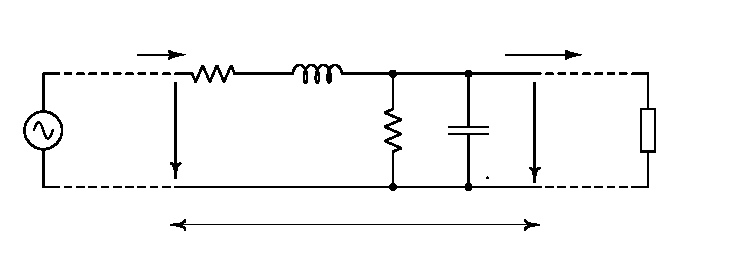
\includegraphics[scale=1.25]{vedenie}\\
   % translate x=237 y=229 scale 0.28
   \putbox{2.43in}{1.52in}{1.20}{\llaL}%
   \putbox{4.00in}{1.64in}{1.20}{\llaidi}%
   \putbox{1.52in}{1.52in}{1.20}{\llaR}%
   \putbox{3.25in}{0.97in}{1.20}{\llaG}%
   \putbox{3.88in}{0.97in}{1.20}{\llaC}%
   \putbox{0.42in}{0.81in}{1.20}{\llaGen}%
   \putbox{5.38in}{0.81in}{1.20}{\llaZat}%
   \putbox{4.36in}{0.81in}{1.20}{\llaudu}%
   \putbox{1.36in}{0.81in}{1.20}{\llau}%
   \putbox{1.09in}{1.64in}{1.20}{\llai}%
   \putbox{2.58in}{0.14in}{1.20}{\lladx}%
   } % close 'parbox'
   } % close 'scalebox'
   \vspace{-\baselineskip} % this is not necessary, but looks better
